% !TEX encoding = UTF-8 Unicode
% лекции 11-12, 19 марта 2016
% конец первой части
% вопросы 21-26
% 21. Теоремы о среднем для гармонических функций
% 22. Сильный принцип максимума для гармонических функций, его следствия. Внутренняя задача Дирихле для уравнения Пуассона. Единственность классического решения
% 23. Обратная теорема о среднем
% 24. Бесконечная дифференцируемость гармонических функций
% 25. Оценки производных гармонических функций. Функции, гармонические во всем пространстве. Теорема Лиувилля.
% 26. Функция Грина внутренней задачи Дирихле для уравнения Пуассона. Функция Грина для шара

\section{Гармонические функции}
\begin{definition} Пусть $\Omega \subset \real^n$ --- область. Функция называется гармонической в $\Omega$, если она является классическим решением уравнения Лапласа:
$$-\Delta u = 0, \quad u \in C^2(\Omega)$$
\end{definition}
\begin{note}
Очевидно, в $\real$ функция будет гармонической тогда и только тогда, когда она линейна.
\end{note}

\subsection{Свойства гармонических функций}
\begin{note}
Пусть $\Omega \subset \real^n$ --- ограниченная область, а $u \in C^2(\Omega)\cap C(\overline{\Omega})$ - гармоническая. Тогда 
$$0 = \int \limits_\Omega \Delta \, u dx = -\int \limits_\Omega \underbrace {\nabla 1}_{0} \cdot \nabla u dx + \int \limits_{\partial\Omega} 1 \cdot \dfrac{\partial u}{\partial \nu}d\sigma\,\Rightarrow\, \int\limits_{\partial\Omega}\dfrac{\partial u}{\partial \nu}d\sigma = 0.$$
Дадим физическую интерпретацию этому замечанию. Уравнение Лапласа задаёт стационарное температурное поле без источников и стоков теплоты. Чтобы такое поле существовало, необходимо, чтобы суммарный поток тепла через границу области должен быть равен нулю.
\end{note}

\begin{theorem}[о среднем для гармонических функций]
Пусть $\Omega \subset \real^n$, $n > 2$, $u$ --- гармоническая в $\Omega$, тогда для любого $x_0 \in \Omega$ верно следующее:
$$u(x_0) = \fint \limits_{\partial B_\eps(x_0)} u(x) d\sigma(x) = \fint \limits_{B_\eps(x_0)} u(x)dx, \quad \forall \eps > 0 \,:\, \overline{B}_\eps(x_0)\subset\Omega.$$
То есть, значение гармонической функции в точке равно как среднему по границе шара, так и среднему по шару с центром в этой точке для любого шара в $\Omega$.
\end{theorem}

\begin{proof}Для начала докажем первое равенство. Пользуясь третьей формулой Грина, получаем

\begin{align*}
u(x_0) & = \int \limits_{\partial B_{\eps}(x_0)} \Phi(x-x_0) \pder[u]{\nu} d\sigma - \int \limits_{\partial B_{\eps}(x_0)} u \pder[\Phi]{\nu} d\sigma - \underbrace {\int \limits_{B_{\eps}(x_0)} \Delta u \Phi (x-x_0) dx}_{=0} = \\
& = \frac {1} {n(n-2)\omega_n}\left(\int \limits_{\partial B_{\eps}(x_0)} \frac {1} {\abs{x - x_0}}^{n-2} \pder[u]{\nu} d \sigma - \int \limits_{\partial B_{\eps}(x_0)} u \pder[]{\nu}\left(\frac {1} {\abs{x-x_0}^{n-2}}\right) d \sigma \right) = \\
& = \frac {1} {n(n-2)\omega_n} \left( \frac {1} {\eps^{n-2}} \underbrace {\int \limits_{\partial B_{\eps}(x_0)} \pder[u]{\nu} d \sigma}_{=0 \text{ по замечанию}} - \int \limits_{\partial B_{\eps}(x_0)} u \frac {n-2} {\eps^{n-1}} d \sigma  \right) = \\
& = \frac {1} {n \omega_n \eps^{n-1}} \int \limits_{\partial B_{\eps} (x_0)} u d \sigma = \fint \limits_{\partial B_{\eps} (x_0)} u d \sigma.
\end{align*}
Первое равенство доказано. Докажем второе. Перепишем интеграл по шару в сферической системе координат:
\begin{align*}
\int \limits_{B_{\eps} (x_0)} u dx &= \int \limits_0^\eps r^{n-1} dr \int \limits_{\partial B_1 (0)} u(\underbrace {x_0 + rs}_{=z}) d \sigma(s) = \int \limits_0^\eps dr \underbrace {\int \limits_{\partial B_r (x_0)} u(z) d \sigma(z)}_{\text{площадь поверхности } \cdot u(x_0)} = \\
& = \int \limits_0^\eps u(x_0) \sigma(\partial B_r(x_0)) dr = u(x_0) \abs{B_\eps (x_0)}.
\end{align*}
Итого,
$$u(x_0) = \fint \limits_{B_{\eps} (x_0)} u dx.$$

\end{proof}

\begin{note}
При $n = 2$ счёт происходит аналогично.
\end{note}

\begin{note}
Пусть $u \in C(\overline{\Omega})$ (непрерывна вплоть до границы). Тогда если есть шар $B_{\eps_0}$, касающийся границы $\Omega$, то утверждение теоремы верно для $\eps \leq \eps_0$. 
\end{note}
\begin{proof}
Пользуясь непрерывностью $u$, переходим к пределу.

\end{proof}

\begin{theorem}[Обратная теорема о среднем]
Пусть $\Omega \subset \real^n$ --- область, $u \in C(\Omega)$. Если для любого шара $B_\rho (x_0)$, замыкание которого лежит в $\Omega$, выполняется
$$ u(x_0) = \fint \limits_{B_\rho(x_0)} u(x) dx,$$
то $u$ --- гармоническая. 
\end{theorem}
\begin{note}
Пусть выполняются условия теоремы, тогда $u$ удовлетворяет соотношению
$$ u(x_0) = \fint \limits_{\partial B_\rho(x_0)} u(x) d\sigma(x)$$
\end{note}
\begin{proof}[Доказательство первого замечания]
Снова воспользуемся сферическими координатами:
$$u(x_0) \cdot \abs{B_\rho (x_0)} = \int \limits_{B_\rho (x_0)} u(x) dx = \int \limits_0^\rho dr \int \limits_{\partial B_r (x_0)} u(z) d \sigma(z).$$
В то же время
$$ u(x_0) \cdot \abs{B_\rho (x_0)} = u(x_0) \cdot \omega_n \rho^n.$$
Приравняем и продифференцируем по $\rho$:
$$ u(x_0) \cdot \underbrace {\omega_n n \rho^{n-1}}_{= \sigma(\partial B_\rho (x_0))} = \int \limits_{\partial B_\rho (x_0)} u(z) d\sigma(z).$$
Итого
$$ u(x_0) = \fint \limits_{\partial B_\rho (x_0)} u(z) d\sigma(z).$$

\end{proof}

\begin{note}
Теорема верна в предположении, что $u \in C^2 (\Omega)$.
\end{note}
\begin{proof}[Доказательство второго замечания]
Дифференцируем соотношение из условия теоремы по $\rho$:
\begin{align*}
0 &= \frac {d} {d\rho} \left( \frac {1} {n \omega_n \rho^{n-1}} \int \limits_{\partial B_\rho (x_0)} u(x) d\sigma(x) \right) = 
 \frac {d} {d\rho} \left( \frac {1} {n \omega_n} \int \limits_{\partial B_1(0)} u(x_0 + \rho s) d\sigma(s) \right) = \\
&= \frac {1} {n \omega_n} \int \limits_{\partial B_1 (0)} \nabla u(x_0 + \rho s) \cdot s d\sigma(s) = 
 \frac {1} {n \omega_n} \int \limits_{\partial B_1 (0)} \pder[u]{s}(x_0 +\rho_s) d\sigma(s) = \\
&= \frac {1} {n \omega_n \rho^{n-1}} \int \limits_{\partial B_\rho (x_0)} \pder[u]{n}(z) d\sigma(z) = 
 \frac {1} {n \omega_n \rho^{n-1}} \int \limits_{B_\rho (x_0)} \Delta u (z) dz = 0, \quad \forall \rho
\end{align*}
Таким образом,
$$\Delta u(x_0) = 0, \quad \forall x_0 \in \Omega$$

\end{proof}

\begin{proof}[Доказательство теоремы]
Имеем функцию $u \in C(\Omega)$. Сгладим её. Для начала рассмотрим функцию
$$ \psi \in C_0^{\infty} (\real), \quad \psi(-x) = \psi(x), \quad \int \limits_{\real} \psi = 1, \quad \supp \psi \subset B_1(0).$$
Теперь введём аппроксимативную единицу $\varphi_\eps$:
$$ \eps >0, \quad \varphi_\eps(x) = \frac {1} {\eps^n} \psi (\frac {\abs{x}} {\eps}). $$
Определим $u_\eps$:
$$ u_\eps = u * \varphi_\eps$$
Заметим, что $u_\eps$ определена не на всём $\Omega$, а только на его подмножестве $\Omega_\eps$, расстояние от которого до границы $\Omega$ равно $\eps$. % здесь можно вставить рисунок

Распишем $u_\eps(x)$:
\begin{align*}
	u_\eps (x) &= \int \limits_{\real^n} u(y) \varphi_\eps (x-y) \, dy = \int \limits_{B_\eps (x)} u(y) \varphi_\eps (x-y) \, dy = \\
	&= \int \limits_0^\eps \, dr \int \limits_{\partial B_r (x)} u(y) \varphi_\eps (x-y) \, d\sigma(y) = \int \limits_0^\eps \, dr \int \limits_{\partial B_1 (0)} u(x+rs) \varphi_\eps (rs) r^{n-1} \, d\sigma(s)
\end{align*}
Функция $\varphi_\eps$ радиальна, значит, можем вынести её за интеграл по $d\sigma(s)$:
\begin{align*}
	u_\eps (x) &= \int \limits_0^\eps r^{n-1} \frac {\psi (\frac {r} {\eps})} {\eps^n} \, dr \int \limits_{\partial B_1 (0)} u(x+rs) \, d\sigma(s) = \int \limits_0^\eps \frac {\psi(\frac {r} {\eps})} {\eps^n} \, dr \int \limits_{\partial B_r(x)} u(z) \, d\sigma(z) =  \\% по первому замечанию 
	&= \int \limits_0^\eps \frac {\psi (\frac {r} {\eps})} {\eps^n} u(x) \omega_n n r^{n-1} \, dr = u(x) \underbrace {\int \limits_0^\eps \frac {r^{n-1}} {\eps^n} \psi \left( \frac {r} {\eps} \right) \omega_n n \, dr}_{\int_{\real^n} \varphi_\eps}
\end{align*}
Получили
\begin{align*}
u_\eps (x) &= u(x) \int \limits_{\real^n} \varphi_\eps = u(x) \quad \text{на } \Omega_\eps \, \forall \eps 
\end{align*}
% уточнить
% u_\eps \in C_0^\infty
\end{proof}

\begin{corollary}
Если $u$ --- гармоническая в $\Omega$, то $u \in C^{\infty} (\Omega)$.
\end{corollary}

\begin{corollary}
Любая производная гармонической функции --- тоже гармоническая функция.
\end{corollary}

\begin{corollary} Пусть $u$ - гармоническая, тогда
$$\abs{D^{\alpha} u(x)} \leq \frac {C_n^{\abs{\alpha}}} {r^{\abs{\alpha}}} \max_{B_r (x)} u(x).$$
\end{corollary}
\begin{proof}
По теореме о среднем:
$$ u_{x_i} (x) = \frac {1} {\omega_n r^n} \int \limits_{B_r (x)} u_{x_i} (x) = \frac {1} {\omega_n r^n} \int \limits_{\partial B_r (x)} u n_i \, d\sigma.$$
Тогда
$$ \abs{u_{x_i} (x)} \leq \frac {1} {\omega_n r^n} n \omega_n r^{n-1} \max_{B_r (x)} u(x) = \frac {n} {r} \max_{B_r (x)} u(x).$$
Для произвольного мультииндекса $\alpha$ оценивание можно проделать соответствующее количество раз, тогда:
$$ \abs{D^{\alpha} u(x)} \leq \frac {C_n^{\abs{\alpha}}} {r^{\abs{\alpha}}} \max_{B_r (x)} u(x).$$

\end{proof}

\begin{note}
В частности, если $u$ ограничена в $\overline \Omega$, то
$$ \abs{D^{\alpha} u(x)} \leq \frac {C_n^{\abs{\alpha}}} {d(x, \partial \Omega)^{\abs{\alpha}}} \max_{\overline{\Omega}} u.$$
\end{note}

\begin{definition}
Функция называется вещественно аналитической, когда она представима в виде своего ряда Тейлора в окрестности всякой точки. При этом в каждой точке ряд равномерно сходится.
\end{definition}
\begin{corollary}
Если $u$ --- гармоническая, то она вещественно аналитическая.
\end{corollary}
\begin{proof}
Запишем ряд Тейлора:
$$ \sum \limits_\alpha \frac {D^{\alpha} u(x_0)} {\abs{\alpha}!} (x - x_0)^{\alpha}, \quad (x-x_0)^{\alpha} = \prod \limits_{i \in 1:n} (x^{(i)} - x_0^{(i)})^{\alpha_i}.$$
Будет ли этот ряд сходиться? Возьмём $x$:
$$ x \in B_r (x_0), \quad \abs{(x-x_0)^{\alpha}} \leq r^{\abs{\alpha}},$$
тогда каждая производная оценивается как
$$ \frac {\abs{D^\alpha u(x_0) \cdot (x-x_0)^\alpha}} {\abs{\alpha}!} \leq \frac {C_n^{\abs{\alpha}}} {\abs{\alpha}!} \max_{\overline{B}_r (x_0)} u(x),$$
а весь ряд можно оценить таким образом:
$$ \sum \limits_\alpha \frac {D^{\alpha} u(x_0)} {\abs{\alpha}!} (x - x_0)^{\alpha} \leq \max_{\overline{B}_r (x_0)} u(x) \cdot \underbrace {\sum_\alpha \frac {C_n^{\abs{\alpha}}} {\abs{\alpha}!}}_{\text{сходится}}.$$

\end{proof}

\begin{note}
Класс вещественно аналитических функций меньше класса бесконечно дифференцируемых функций.
\end{note}

\begin{note}
Если вещественно аналитическая функция равна 0 на каком-то интервале, то она равна нулю всюду.
\end{note}

\begin{corollary}[Теорема Лиувилля]
Пусть $\Omega = \real^n$, а функция $u$ --- гармоническая и ограниченная. Тогда $u \equiv \const$.
\end{corollary}
\begin{proof}
Воспользуемся предыдущим следствием:
$$ \abs{u_{x_i} (x_0)} \leq \frac {C_n} {r} \sup_{\real^n} u(x) \quad \forall r$$
Устремив $r$ к бесконечности, получаем
$$ \abs{u_{x_i} (x_0)} = 0 \quad \forall x_0 \, \forall i$$
Значит, $\nabla u = 0$, и, как следствие, $u \equiv \const$.

\end{proof}

\begin{theorem}[Принцип максимума]
Пусть $\Omega$ --- связная область, а $u$ --- гармоническая в ней. Если
$$ \exists \, x_0 \in \Omega: \, u(x_0) = \sup_\Omega u(x),$$
 то $$u \equiv u(x_0).$$
\end{theorem}
\begin{proof}
Пусть такая точка $x_0$ существует. Представим $\Omega$ в виде дизъюнктного объединения $A_1$ и $A_2$:
\begin{align*}
	A_1 &:= \left\{ x \in \Omega: \, u(x) = u(x_0) \right\} \neq \varnothing, \\
	A_2 &:= \left\{ x \in \Omega: \, u(x) < u(x_0) \right\} = \Omega \setminus A_1.
\end{align*}
Пусть $A_2$ тоже непусто (иначе утверждение теоремы тривиально). Вспомним, что прообраз замкнутого множества замкнут. Заметим, что $A_1$ --- прообраз замкнутого множества $\left\{ u(x_0) \right\}$. Значит, $A_1$ --- замкнутое, откуда следует, что $A_2$ открыто.
% относительно замкнуто\footnote{ непрерывный образ замкнутого множества замкнут} в $\Omega$

Теперь покажем, что $A_1$ открыто. Возьмём некоторую точку $z \in A_1$ и шар $B_r (z)$ такой, что он не касается границы $\Omega$. Тогда весь шар находится внутри $A_1$. Допустим, это не так. Тогда в какой-то точке $y \in B_r (z) $ значение $u(y) < u(x_0)$ и среднее по этому шару будет меньше, чем $u(x_0)$. Но по теореме о среднем оно должно быть равно $u(z) = u(x_0)$. Значит, любой шар $B_r (z)$ лежит в $A_1$. Следовательно, $A_1$ --- открытое.
% TODO: написать получше, сейчас рассуждения просто сливаются

Мы пришли к тому, что $\Omega$ разбивается на два непересекающихся открытых множества, что противоречит связности. Значит, $A_2$ --- пусто, и $A_1 = \Omega$.

\end{proof}

\begin{note} Заменой $u$ на $-u$ и супремума на инфимум получается принцип минимума.
\end{note}

\begin{corollary} Пусть $\Omega$ --- ограниченная область в $\real^n$ и поставлена задача Дирихле для уравнения Пуассона:
\begin{align*}
	\begin{cases*}
		- \Delta u = f,\\
		u\Big\rvert_{\partial \Omega} = u_0.
	\end{cases*}
\end{align*}
Тогда если классическое решение
$$ u \in C^2(\Omega) \cap C(\overline{\Omega})$$
существует, то оно единственно.
\end{corollary}
\begin{proof}
Следует из принципа максимума. Пусть есть два решения $u_1$ и $u_2$, тогда $u = u_1 - u_2$ --- решение задачи
\begin{align*}
	\begin{cases*}
		- \Delta u = 0,\\
		u\Big\rvert_{\partial \Omega} = 0.
	\end{cases*}
\end{align*}
Получается, что $u$ --- непрерывная вплоть до границы гармоническая функция. Значит, она имеет и максимум, и минимум. Далее возможны два случая:
\begin{enumerate}
\item Максимум достигается внутри области. Тогда внутри каждой компоненты связности $u \equiv const$, но при этом имеем $0$ на границе. Значит, $u \equiv 0$.
\item Максимум и минимум достигаются на границе. Там она $0$. Значит, $u \equiv 0$.
\end{enumerate}
\end{proof}

\section{Функция Грина внутренней задачи Дирихле для уравнения Пуассона}
\subsection{Формулы Грина}
Пусть $\Omega \subset \real^n$ --- ограниченная область с гладкой границей. Тогда верны формулы Грина:
\begin{enumerate}
\item $\displaystyle \int \limits_\Omega v \Delta u = - \int \limits_\Omega \nabla v \cdot \nabla u \, dx + \int \limits_{\partial \Omega} v \pder[u]{n} \, d\sigma,$
\item $\displaystyle \int \limits_\Omega u \Delta v - v \Delta u = \int \limits_{\partial \Omega} u \pder[v]{n} - v \pder[u]{n} \, d\sigma,$
\item $\displaystyle u(x_0) = \int \limits_{\partial \Omega} \Phi (x-x_0) \pder[u]{n} \, d\sigma - \int \limits_{\partial \Omega} u \pder[\Phi]{n} (x-x_0) \, d\sigma - \int \limits_\Omega \Delta u \Phi (x - x_0) \, dx,$
\end{enumerate}
где 
$$ \Phi(x) = \frac {1} {n (n-2) \omega_n} \cdot \frac {1} {\abs{x}^{n-2}}$$
--- фундаментальное решение уравнения $$-\Delta \Phi = \delta.$$

\subsection{Определение}
Пусть $\Omega \subset \real^n$ --- ограниченная область с гладкой границей, $u \in C^2(\Omega) \cap C(\overline{\Omega})$. Рассмотрим уравнение Пуассона в $\Omega$:
\begin{align*}
	\begin{cases*}
		- \Delta u = f, \\
		u\Big\rvert_{\partial \Omega} = u_0.
	\end{cases*}
\end{align*}
Будем искать функцию
$$G: \, \Omega \times \Omega \rightarrow \real$$ вида
$$G(x,y) = \Phi (x-y) + v^y (x),$$
где
\begin{gather*}
	- \Delta v^y = 0 \quad \text{в $\Omega$} \\
	\begin{cases*}
		- \Delta_x G(x,y) = \delta_y \\
		G(x,y)\Big\rvert_{x \in \partial \Omega} = 0.
	\end{cases*}
\end{gather*}
\begin{definition}
Функция $G(x,y)$ называется функцией Грина задачи Дирихле и зависит только от области $\Omega$.
\end{definition}

Физический смысл таков: пусть $y$ фиксирована, тогда $G(x,y)$ --- потенциал электростатического поля единичного заряда в точке $y$ при заземлённой границе $\Omega$.

Условия на $v^y$ таковы:

\begin{align*}
	\begin{cases*}
		- \Delta v^y = 0 \\
		v^y\Big\rvert_{\partial \Omega} = - \Phi(x-y)\Big\rvert_{x \in \partial \Omega}.
	\end{cases*}
\end{align*}

Функция $\Phi(x-y)$ --- потенциал поля заряда в точке $y$ в открытом пространстве. А если поставить сюда железную границу (заземлить), то потенциал изменится. Создастся некий дополнительный заряд, компенсирующий потенциал, создаваемый зарядом $y$ в открытом пространстве.

Значит, $v^y$ --- потенциал собственной системы, компенсирующей заряд. На поверхности $\Omega$ он будет равен минус потенциалу, созданному электростатическим полем от заряда в точке $y$ в свободном пространстве.

Предположим, что $v^y$ удалось найти. Запишем третью формулу Грина:
$$ u(y) = \int \limits_{\partial \Omega} \pder[u]{n} \Phi (x-y) - u \pder[\Phi(x-y)]{n_x} \, d\sigma(x) - \int \limits_\Omega \Phi (x -y) \Delta u(x) \, dx.$$
Запишем вторую формулу Грина для $v^y$:
$$ \int \limits_{\partial \Omega} v^y \pder[u]{n} - u \pder[v^y]{n} \, d\sigma - \int \limits_\Omega v^y \Delta u \, dx = \int \limits_{\Omega} u \underbrace{\Delta v^y}_{ = 0} \, dx = 0.$$
Сложим:
\begin{align*}
	u(y) & = \int \limits_{\partial \Omega} \pder[u]{n} \underbrace{(v^y + \Phi (x-y))}_{=G(x,y)} - u \pder{n_x} (\Phi (x-y) + v^y) \, d\sigma - \int \limits_\Omega (\Phi (x-y) + v^y) \Delta u \, dx = \\
	& = \int \limits_{\partial \Omega} \pder[u]{n} \underbrace{G(x,y)}_{=0} - u \pder{n_x} G(x,y) \, d\sigma - \int \limits_\Omega G(x,y) \Delta u \, dx = \\
	& = - \int \limits_{\partial \Omega} u \pder{n_x} G(x,y) \, d\sigma(x) - \int \limits_\Omega G(x,y) \Delta u \, dx.
\end{align*}
Таким образом, решение задачи Дирихле выражается интегральной формулой:
$$ u(y) = - \int \limits_{\partial \Omega} u_0(x) \pder{n_x} G(x,y) \, d\sigma(x) + \int \limits_\Omega G(x,y) f(x) \, dx.$$
Это верно, если мы смогли найти такую $G(x,y)$.

\begin{note} На самом деле, можно доказать существование функций Грина для довольно широкого класса областей, но мы не будем этим заниматься.
\end{note}

\subsection{Общие свойства}
Пусть $\Omega \subset \real^n$ --- ограниченная область, и функция $G(x,y)$ для $\Omega$ существует. Тогда:

\begin{enumerate}
\item $G(x,y) \geq 0$ всюду. 
\begin{proof} Вырежем из $\Omega$ небольшой шар $B_\eps (y)$.

\begin{center}
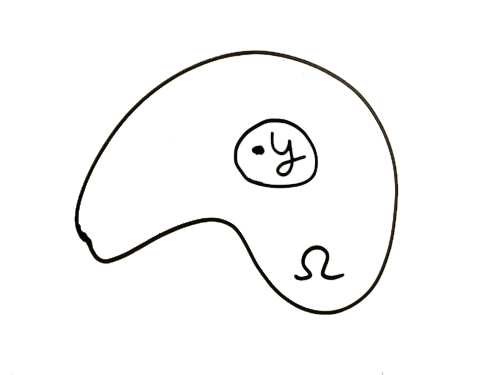
\includegraphics[scale=0.3]{part6.1.png}
\end{center}

В множестве $\Omega \setminus B_\eps (y)$ функция Грина будет гармонической. Для достаточно маленького $\eps$ будет верно

\begin{align*}
	\begin{cases*}
		- \Delta_x G(x,y) = \delta_y, \\
		G(x,y)\Big\rvert_{x \in \partial \Omega} = 0.
	\end{cases*}
\end{align*}
При достаточно маленьком $\eps$ имеем
$$ G(x, y) = \underbrace{\Phi(x-y)}_{\substack{\text{сколь угодно} \\ \text{большая}}} + \underbrace{v^y(x)}_{\substack{\text{гармоническая,} \\ \text{ограниченная}}} \quad \Rightarrow \quad G(x,y)\Big\rvert_{\partial B_\eps (y)} > 0.$$
Функция $G(x,y)$ достигает максимума и минимума на границах, а на границах она неотрицательна. Значит, она неотрицательна всюду.
% как-то хлипко вышло

\end{proof}
\item $ \displaystyle \lim_{x \to y} G(x,y) = + \infty$.
\begin{proof}Видно из доказательства предыдущего свойства.

\end{proof}
\item $G(x, y) = G(y, x)$ --- функция Грина симметрична.
\begin{proof}
Пусть
$$ u(x) = G(x,y), \quad v(x) = G(x,z).$$
Рассмотрим два непересекающихся шара $U(y) \subset \Omega$ и $V(z) \subset \Omega$.

\begin{center}
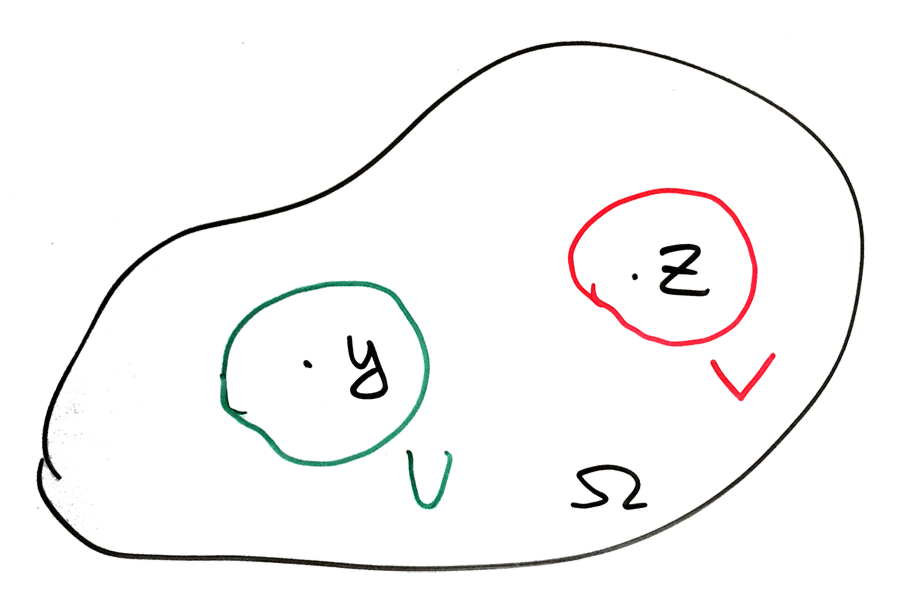
\includegraphics[scale=0.2]{part6.2.png}
\end{center}

Заметим, что верно
\begin{align*}
	- \Delta u = 0\quad \text{в $V$}, \\
	- \Delta v = 0 \quad \text{в $U$}. 
\end{align*}
По второй формуле Грина для $\Omega \setminus (U \cup V)$:
$$ \int \limits_\Omega \underbrace{u \Delta v - v \Delta u}_{=0} \, dx = \int \limits_{\partial U} u \pder[v]{n} - v \pder[u]{n} \, d\sigma + \int \limits_{\partial V} u \pder[v]{n} - v \pder[u]{n} \, d\sigma = 0.$$

Тогда по третьей формуле Грина
\begin{align*}
	v(y) = - \int \limits_{\partial U} u \pder[v]{n} - v \pder[u]{n} \, d\sigma \quad \text{в $U$}, \\
	u(z) = - \int \limits_{\partial V} v \pder[u]{n} - u \pder[v]{n} \, d\sigma \quad \text{в $V$}.
\end{align*}
Подставим последние две формулы в формулу до них:
$$ -v(y) + u(z) = 0 \quad \Rightarrow \quad G(y,z) = G(z,y).$$

\end{proof}

\end{enumerate}

\subsection{Нахождение функции Грина для полупространства}
Для начала рассмотрим $\Omega = \left\{ x_n > 0 \right\} \subset \real^n$ --- полупространство.
\begin{note}
Представим, что мы находимся в 18 веке: не будем обращать внимания на формальности, говорящие, что область $\Omega$ должна быть ограниченной.
\end{note}
В нижнем полупространстве находится "земля" (потенциал равен нулю). Поместим заряд в $1$ Кл в точку $y$. Требуется посчитать его потенциал.

Такую задачу можно свести к задаче без заземления: представим, что заземления нет. Далее поставим заряд в $-1$ Кл в точку $y'$, симметричную относительно границы нашего полупространства, и будем рассматривать эту систему.

\begin{center}
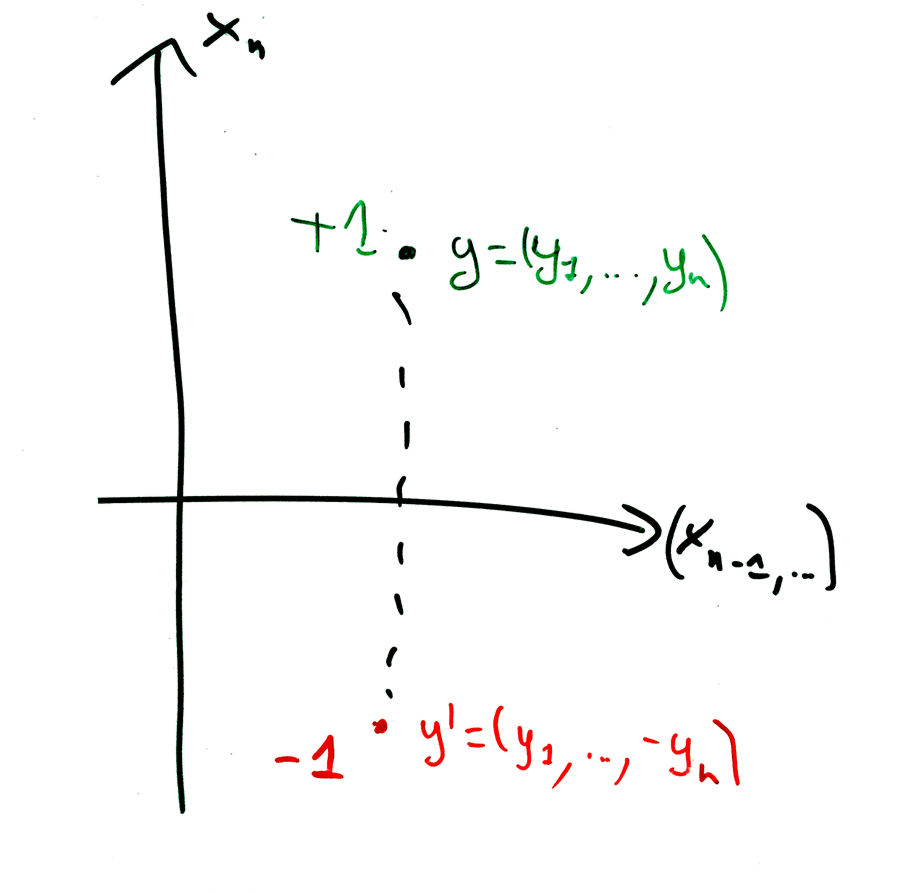
\includegraphics[scale=0.25]{part6.3.png}
\end{center}

Тогда
$$ G(x,y) = \Phi (x-y) - \Phi (x - y'),$$
где
$$ \Phi (x - y) = \frac {1} {n (n-2) \omega_n} \frac {1} {\abs{x-y}^{n-2}}.$$
По геометрическим соображениям потенциал этой системы зарядов на границе полупространства будет равен нулю. В некотором определённом смысле с помощью полученной $G(x,y)$ можно решить задачу Дирихле в полупространстве.

\subsection{Нахождение функции Грина для шара}
Перейдём к шару. Для простоты наш шар это $B_1 (0) \subset \real^n$. Допустим, у нас есть заземлённая граница шара и заряд в $1$ Кл в точке $y$. Создадим систему зарядов, в которой при отсутствии заземлённой границы "фиктивные" заряды компенсируют потенциал имеющегося заряда. Делаем инверсию:
$$ y' = \frac {y} {\abs{y}^2}. $$

Воспользуемся свойством инверсии:
$$ (\abs{y} \cdot \abs{x-y'})^2 = \abs{y}^2 (\abs{x}^2 + \abs{y'}^2 - 2 xy') \stackrel{\abs{x}=1}=(\abs{y}^2 + 1 - 2 x y') = \abs{x-y}^2.$$
То есть,
$$ \abs{y} \cdot \abs{x-y'} = \abs{x-y} \quad \text{при } \abs{x} = 1.$$.

\begin{center}
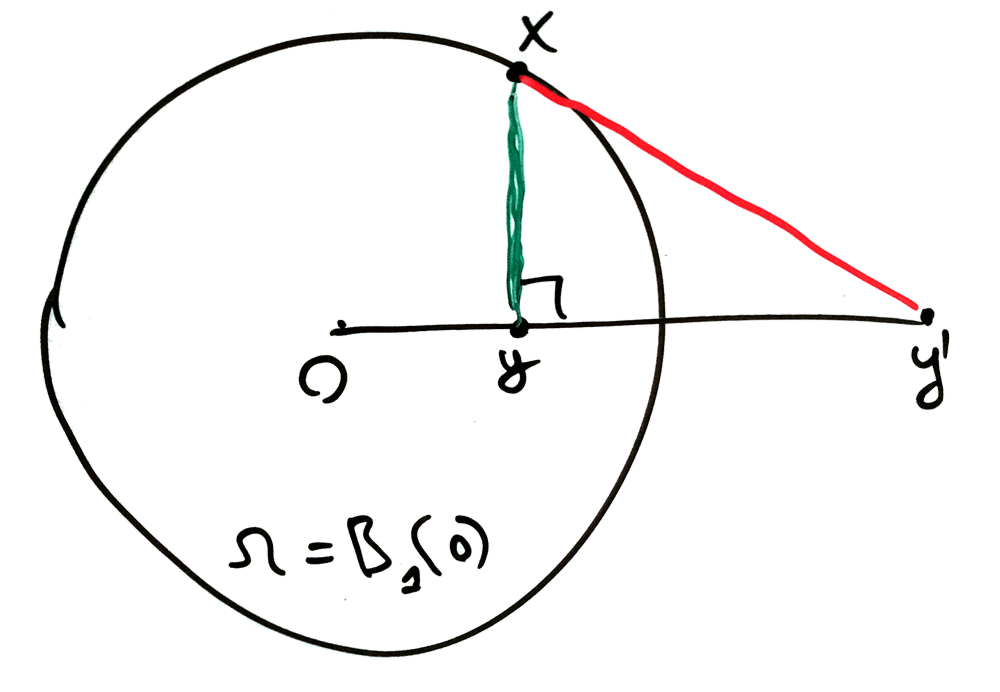
\includegraphics[scale=0.2]{part6.4.png}
\end{center}

Тогда в качестве $G$ возьмём сумму двух кулоновских потенциалов:
$$ G(x,y) = \frac {1} {n (n-2) \omega_n} \left( \frac {1} {\abs{x-y}^{n-2}} - \frac {1} {\abs{y} \cdot \abs{x-y'}^{n-2}} \right).$$
Непосредственно проверяются условия из определения функции Грина:
\begin{align*}
	\begin{cases*}
		- \Delta_x G(x, y) = \delta_y, \\
		G(x, y)\Big\rvert_{\abs{x} = 1} = 0.
	\end{cases*}
\end{align*}
Значит, в результате инверсии мы получили нужный "фиктивный" заряд и нашли функцию Грина для шара. Решим задачу Дирихле для уравнения Лапласа в единичном шаре:

\begin{align*}
	\begin{cases*}
		- \Delta u = 0, \\
		u\Big\rvert_{\partial \Omega} = u_0.
	\end{cases*}
\end{align*}
Считаем:
$$u(y) = - \int \limits_{\partial \Omega} u_0 \pder{n_x} G(x,y) \, d\sigma(x) + \int \limits_\Omega \underbrace{f(x)}_{=0} G(x,y) \, dx = - \int \limits_{\partial B_1 (0)} u_0 k(x, y) \, d\sigma(x),$$
где
$$ k (x,y) = - \pder{n_x} G(x,y) = \frac {1 - \abs{y}^2} {n \omega_n} \frac {1} {\abs{x-y}^n} = - \nabla_x G(x,y) \cdot \underbrace{x}_{\substack{\text{направление} \\ \text{нормали}} } \quad \text{--- ядро Пуассона}.$$

\begin{exercise} Показать, что полученное $u$ --- действительно решение.
\end{exercise}
\begin{note}Так как
% TODO: дописать про пронос лапласиана под знак интеграла
$$- \Delta u(y) = \int \limits_{\partial B_1 (0)} u_0 \Delta_y k(x, y) \, d\sigma,$$
то достаточно доказать, что при фиксированном $x$ функция $k$ --- гармоническая по второй переменной:
$$ - \Delta_y k(x,y) = 0, \quad \abs{x} = 1.$$
\end{note}

\begin{exercise} Показать, что
$$ \lim_{\substack{y \to x_0 \\ \abs{x_0} = 1}} k(x, y) = 0 \quad x_0 \neq x$$
и
$$ k( x, \cdot) \notin C(\overline{\Omega}) \quad \forall x.$$
\end{exercise}

\begin{note}Пусть $Q$ --- матрица поворота. Тогда
$$ u(Qy) = u(y),$$
то есть $u$ радиально симметрична.
\end{note}
\begin{proof}
Посчитаем:
\begin{align*}
	u(Qy) &= \int \limits_{\partial \Omega} \frac {1 - \abs{Qy}^2} {n \omega_n \abs{x-Qy}^n} \, d\sigma(x) = \int \limits_{\partial \Omega} \frac {1 - \abs{y}^2} {n \omega_n \abs{Qx-y}^n} \, d\sigma(x) \stackrel{z = Qx} = \\
	&= \int \limits_{\partial \Omega} \frac {1 - \abs{y}^2} {n \omega_n \abs{z - y}^n} \underbrace {\abs{Q}}_{=1} \, d\sigma(z) = u(y). 
\end{align*}

Мы воспользовались тем, что
\begin{align*}
	\abs{x-Qy}^n = \left( \abs{x-Qy}^2 \right)^{\frac {n} {2}} = (1 + \abs{y}^2 - 2 x Q y)^{\frac {n} {2}} = (1 + \abs{y}^2 - 2Qxy)^{\frac {n} {2}} = \abs{Qx - y}^n
\end{align*}

\end{proof}

\begin{note} $u(y) = 1$.
\end{note}
\begin{proof}
Функция $u$ гармоническая и радиально симметрична. Рассмотрим сферы с центром в нуле и с $y$ на границе:
\begin{center}
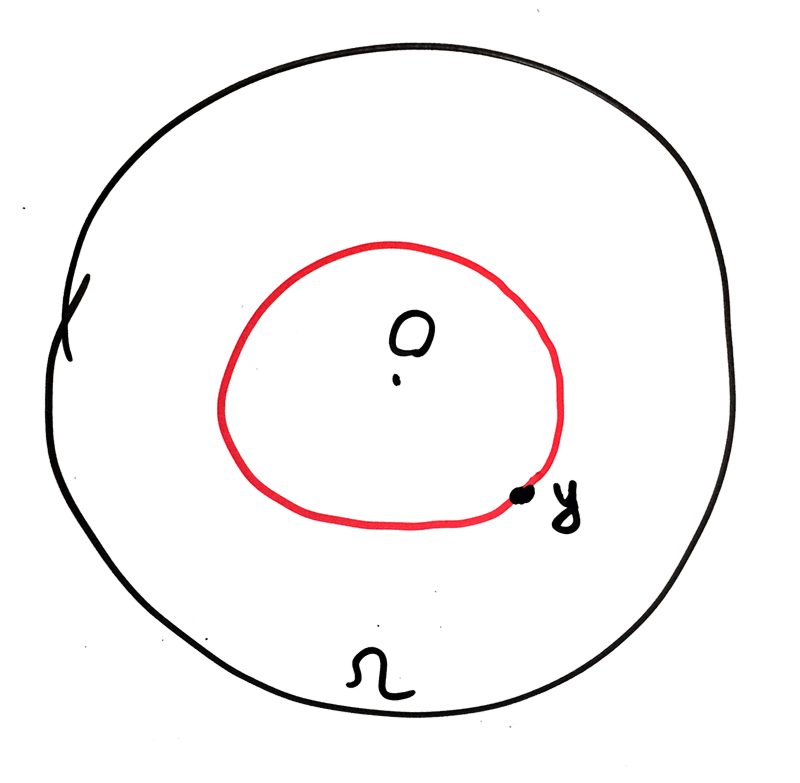
\includegraphics[scale=0.2]{part6.5.png}
\end{center}
На каждой такой сфере функция $u$ константна. По теореме о среднем функция в нуле равна среднему по любой такой сфере. Значит, она константна везде и равна значению в центре:
$$ u(y) = u(0) = \frac {1} {n \omega_n} \int \limits_{\partial B_1 (0)} \frac {1} {\abs{x}^n} \, d\sigma = 1.$$

\end{proof}

\begin{note}
$$\lim_{y \to x_0} u(y) = u_0 (x_0).$$
\end{note}
\begin{proof}
Посчитаем:
\begin{align*}
	|u(y) - u_0(x_0)| &= \left| \, \int \limits_{\partial \Omega} k(x, y) u_0(x) \, d\sigma(x) - u_0(x_0) \int \limits_{\partial \Omega} k(x,y) \, d\sigma(x) \right| = \\
	& = \left| \, \int \limits_{\partial \Omega} k(x,y) (u_0(x) - u_0(x_0)) \, d\sigma(x)\right| \leq \\
	& \leq \int \limits_{\partial \Omega} k(x, y) | u_0(x) - u_0(x_0) | \, d\sigma(x) \leq \\
	& \leq \int \limits_{\partial \Omega \cap B_\eps (x_0)} k(x, y) \delta \, d\sigma(x) + 2 || u_0 ||_\infty \int \limits_{\partial \Omega \setminus B_\eps (x_0)} k(x, y) \, d\sigma(x),
\end{align*}
где 
$$ \eps: \, |x - x_0| \leq \eps \Rightarrow |u_0(x) - u_0(x_0)| \leq \delta $$
и
$$ |u_0 (x) - u_0(x_0)| \leq 2 || u_0 ||_\infty.$$
Знаем, что 
$$ \lim_{y \to x_0} k(x, y) = 0 \quad \text{и} \quad \int \limits_{\partial \Omega \cap B_\eps (x_0)} \leq 1,$$
значит,
$$ \lim_{y \to x_0} |u(y) - u_0(x_0)| \leq \delta \cdot 1 + 0 \quad \forall \eps$$

\end{proof}

\section{Упражнения}

Список полезных упражнений для подготовки к коллоквиуму.

\begin{enumerate}
\item  Докажите, что оператор Лапласа не меняет форму при повороте системы координат (проделать вычисления в $\real^2$).
\item Докажите, что оператор Даламбера $u\mapsto u_{tt} - u{xx}$, $x\in \real$ не меняет форму при гиперболическом повороте системы координат $(x,t)$.
\item Как выглядит оператор Лапласа в цилиндрической системе координат? В сферической системе координат? Найти радиально­симметричные гармонические функции в шаре в $\real^3$, в $\real^2$.
\item Найти первые и вторые производные обобщенных функций (на $\real$) $|x|$, $2\sign  x + x^2$, $x^+$.
\item * Решить в обобщенных функциях (на $\real$) уравнения $x u = 0$ и $x^2 u=0$ относительно неизвестной $u$. (Кстати: тут написано произведение обобщенной функции на бесконечно дифференцируемую. Как его естественно определить?)
\item Докажите, что функция, гармоническая в области, в окрестности каждой точки области представима сходящимся степенным рядом. Оцените радиус сходимости ряда. Указание: используйте оценки производных гармонической функции (в лекциях обсуждалось, как).
\item Пусть $u$ --- непрерывная ограниченная функция в пространстве $\real^n$. Рассмотрим две произвольные точки $x, y$. Доказать, что средние $u$ по шарам $B_r(x)$, $B_r(y)$ ''почти равны'', если $r>>1$ (т.е. очень большое число). Вывести отсюда теорему Лиувилля для ограниченных гармонических функций.
\item Пусть $\Omega\subset \real^n$ --- ограниченная область, $k$: $\bar\Omega\times\partial\Omega\to \real^+$ --- непрерывная функция, определённая всюду, кроме диагонали $\{x=y\}$, причем $\int_{\partial \Omega}k(\cdot,y)\, d\sigma(y)=1$, и $k(x,y)\to 0$, если $x\to x_0\in \partial \Omega$, равномерно по $y\in B_\delta (x_0)$ (для любого $\delta>0$). Пусть $g$ --- непрерывная функция на $\partial \Omega$. Доказать, что $\int_{\partial \Omega}k(x,y)g(y)\, d\sigma(y) \to g(x_0)$, если $x\to x_0\in \partial \Omega$ (это, собственно, и проделывается в обосновании формулы Пуассона).
\item Пусть $\Phi$ --- ядро теплопроводности в $\real^+\times \real^n$. Доказать, что $\Phi(\eps, x)\to \delta_0$ в смысле обобщенных функций в $\real^n$, если $\eps \to 0^+$.

\end{enumerate}